\section{Einführung}
  \subsection{Anfang des Internets: 60er Jahre}
    \begin{itemize}
      \item 1969: "Geburtsstunde" des Internet
        \begin{itemize}
          \item Die ersten Knoten von ARPAnet sind funktionsfähig: Datenübertragung zwischen vier
            Rechnern in den USA
            \begin{itemize}
              \item University of California at Loa Angeles (UCLA)
              \item Stanford Research Institute (SRI)
              \item University of California at Santa Barbara (UCSB)
              \item University of Utah
            \end{itemize}
          \item Erste Verbindung war zsichen UCLA und SRI
        \end{itemize}
      \item 1972: Öffentliche Demonstration des Internet (ARPAnet) 
        \begin{itemize}
          \item mit 15 Knoten
        \end{itemize}
    \end{itemize}
    \subsubsection{Kritische Infrastruktur}
      Kritische Infrastrukturen sind Systeme, die von wesentlicher Bedeutung zur Aufrechterhaltung
      wichtiger gesellschaftlicher Funktionen, der Gesundheit, der Sicherheit und des wirtschaftlichen
      und sozialen Wohlergehens der Bevölkerung sind.
      \begin{itemize}
        \item Beispiele: Energie, Wasser, Informationstechneik und Telekommunikation ($\ra$ Internet),
          Transport und Verkehr
      \end{itemize}
  \subsection{Begriffsbildung Rechnernetz und Paket}
    \subsubsection{Rechnernetz}
      Ein Rechnernetz besteht aus Komponenten und (Kommunikations-)Links, die diese miteinander
      verbinden
    \subsubsection{Links}
      Links sind Übertragungsmedien (kurz Medien)
      \begin{itemize}
        \item Beispiele für Übertragungsmedien: Koaxialkabel, Glasfaser, Funk
      \end{itemize}
    \subsubsection{Komponenten}
      Komponenten sind Endsysteme oder Zielsysteme
    \subsubsection{Endsysteme}
      Endsysteme (Hosts) führen verteilte Anwengungen aus. Diese benötigen ein Netz zu Kommunikation
      zwischen räumlich verteilten Anwendungsinstanzen.
      \begin{itemize}
        \item Beispiel für verteilte Anwendungen: WhatsApp, Email
        \item Beispiel für Endsysteme: Notebook, Smartphone, Herzschrittmacher, Kühlschrank
      \end{itemize}
    \subsubsection{Zwischensysteme}
      Zwischensysteme leiten Daten im NEtz weiter und führen im Normalfall keine verteile Anwendung aus
      \begin{itemize}
        \item Beispiele für Zwischensysteme: Router, Switch
      \end{itemize}
    \subsubsection{Verschieden große Rechnernetzte}
      \begin{itemize}
        \item Lokales Netz (Local Area Network, LAN)
          \begin{itemize}
            \item Rechnernetz, dessen geographische Ausdehnung auf mehrere Hundert Meter bis wenige
              Kilometer beschränkt ist
            \item Eigentümer ist typischerweise diejenige Organisation, der die Komponenten gehören.
              Sind i.d.R. privat
              Beispiele: Unternehmensnetz, Heimnetz
          \end{itemize}
        \item Weitverkehrsnetz (Wide Area Network, WAN)
          \begin{itemize}
            \item Rechnernetz, das sich über große geographische Distanzen erstrecket
            \item Können privat sein oder öffentlich genutzt werden
            \item Beispiele: Google-Netz zu internen Verbindung von dessen Rechnerzentren, Netz der
              Deutschen Telekom AG
          \end{itemize}
      \end{itemize}
    \subsubsection{(Daten-)Pakete}
      Die von den Anwendungen zu sendenen Daten können in kleiner Teile gegliedert werde. Diese werden
      als (Daten-)Pakete bezeichnet
      \begin{itemize}
        \item Typischer Aufbau von Paketen
          \begin{itemize}
            \item Nutzdaten: die von der Anwendung zu versendenden Daten
            \item Metadaten: für die Steuerung der Protokolle erforderlich
          \end{itemize}
        \item Pakete werden im Netz i.d.R. unabhängig voneinander behandelt
        \item Werden durch das Netz zur Zielanwendung weitergeleitet
          \begin{itemize}
            \item Werden hierzu von Zwischensysteme zu Zwischensystem (hop-by-hop) weitergeleitet
          \end{itemize}
        \item Sind voneinander unabhängige Einheiten für die Weiterleitung
      \end{itemize}
  \subsection{Zentrale Konzepte und Probleme im Networking}
    \begin{itemize}
      \item Layering (Schichtung): Wie kann die Komplexität beherrscht werden? $\ra$ Modularisierung
      \item Naming: Wie können Computer, Dienste und Protokolle angesprochen werden? $\ra$ Adressen,
        Namen
      \item Routing (Wegewahl): Wie werden Wege/Pfade von A nach B gefunden?
      \item Reliability (Zuverlässigkeit): Wie kann man zuverlässig über unzuverlässige Medien
        kommunizieren?
      \item Resource Sharing: Wie knappe Resourcen zwischen konkurrierenden Parteien aufteilen
    \end{itemize}
    \subsubsection{Best-Effort Service}
      Internet =
        \begin{itemize}
          \item Netz-Infrastruktur
            \begin{itemize}
              \item Besteht u.a. aus Routern, Switches und Links
              \item Überträgt Daten zwischen Endsystemen
            \end{itemize}
          \item + Datentransport + Anwendungssoftware
            \begin{itemize}
              \item Auf den Endsystemen
              \item Anwendungssoftware verarbeitet Daten
            \end{itemize}
          \item Paket-basiertes Netz
            \begin{itemize}
              \item Paket: Einheit über Übertragung
                \begin{itemize}
                  \item Menge von Bits (typischerweise $\le$ 1500 Byte)
                  \item Nutzdaten + Metadaten (z.B. Adressen)
                \end{itemize}
            \end{itemize}
          \item Auslieferung der Pakete:
            \begin{itemize}
              \item Kleinster gemeinsamer Nenner für alle Anwendungen
              \item Keine Zusicherung ob, wann und mit welcher Geschwindigkeit
              \item Minimale Anforderung an Netz-Infrastruktur
              \item Anwendungen können sich an performance anpassen
              \item Netzbetreiber können Performance erhöhren (mehr und schnellere Links)
            \end{itemize}
        \end{itemize}
    \subsubsection{Architektur}
      Grundprinzip: Modularisierung
      \begin{itemize}
        \item Kleinere Aufgaben mit klar definierten Schnittstellen
        \item Gliederung in übereinanderliegende Schichten
      \end{itemize}
      Schichten der Netz-Infrastruktur\\\\
      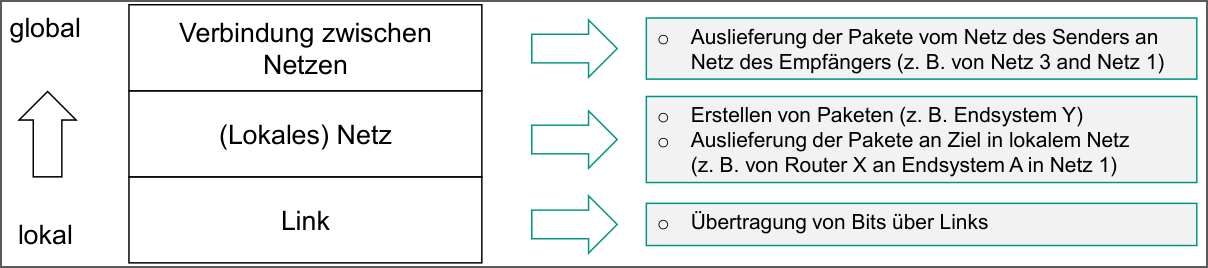
\includegraphics[width=\textwidth]{img/netz_infrastruktur.png}
    \subsubsection{Schichtmodell / Referenzmodell}
      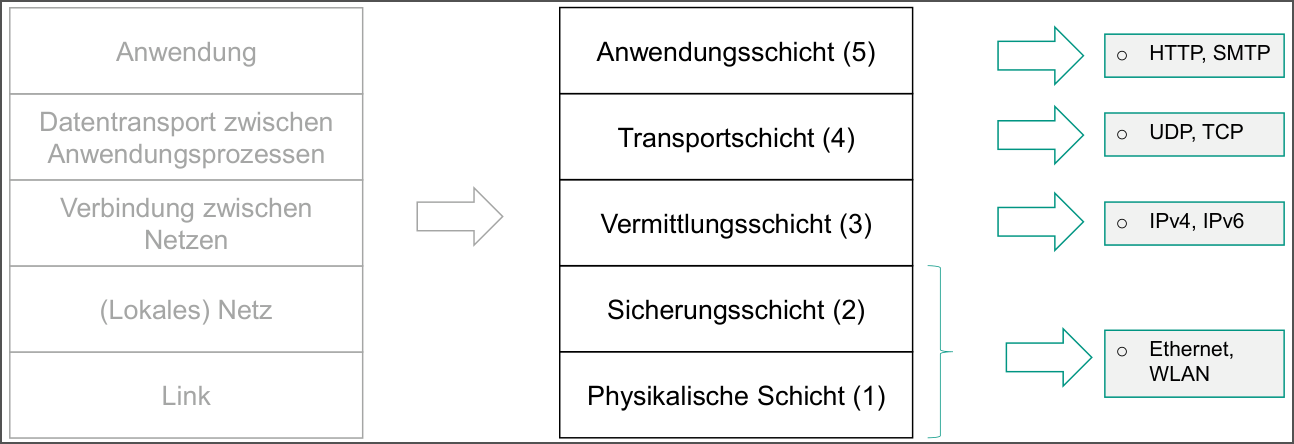
\includegraphics[width=\textwidth]{img/schichtmodell.png}
    \subsubsection{Hourglass-Modell}
      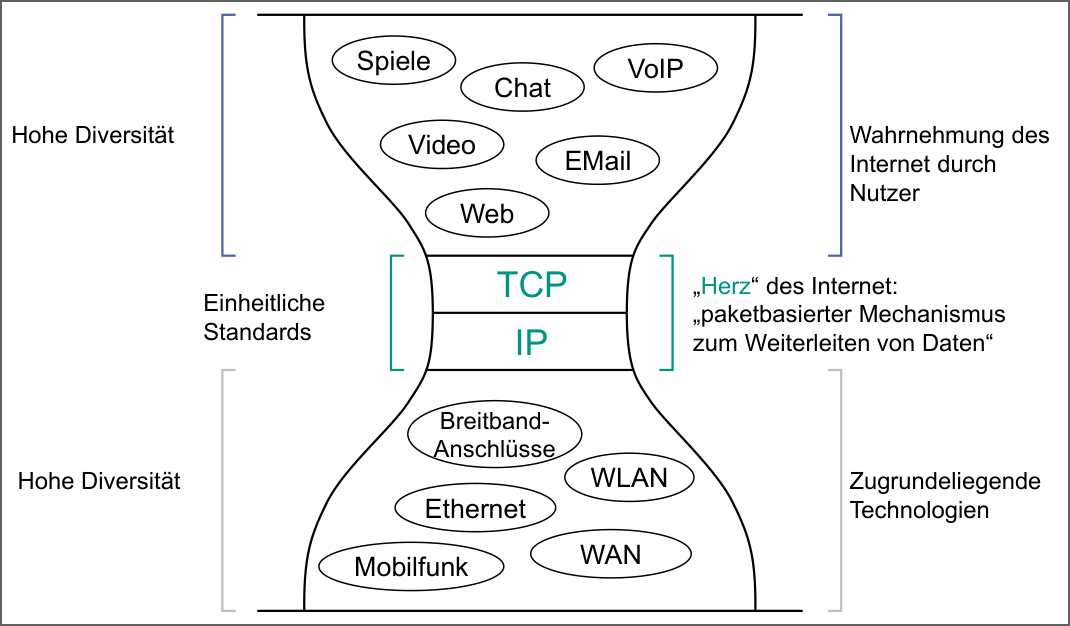
\includegraphics[width=\textwidth]{img/hourglass_modell.png}
      \begin{itemize}
        \item Vermittlungs- und Transportschicht bilden "narrow waist"
          \begin{itemize}
            \item Einheitliche Standards im Internet auf diesen Schichten (Protokolle IP und TCP/UDP)
            \item Separieren Details der Andwendung von Deteils der Technologie
          \end{itemize}
        \item Diversität bei Technologien und Anwendungen unterstützt
          \begin{itemize}
            \item Unterschiedliche Technologien in verschiedenen Netzen, z.B. Mobilkommunikation,
              WLAN, Ethernet
            \item Unterschiedliche Anwendungen, z.B. Email, Messaging, Streaming
          \end{itemize}
      \end{itemize}
    \subsubsection{Routing}
      Wege für Paketweiterleitung zum Ziel finden
      \begin{itemize}
        \item In Netzen (Nutzung von Switches)
        \item Zwischen Netzen (Nutzung von Routern)
        \item Weiterleitungstabelle durch Routingprotokoll etabliert
      \end{itemize}
    \subsubsection{Zuverlässige Auslieferung (Reliable Deliver)}
      Pakete können verloren gehen z.B. durch
      \begin{itemize}
        \item Überlastete Links
        \item Nicht funktionierende Router
      \end{itemize}
      Zuverlässigkeit gefordert, dann
      \begin{itemize}
        \item Sendewiederholungen durch Sender notwendig
        \item Hierzu: Sender muss über Verlust (bzw. nich Verlust) informiert werden
          \begin{itemize}
            \item Quittungen vom Empfänger (z.B. positive Quittung, Acknowledgement (ACK))
            \item Timeout beim Sender wenn keine Quittung zu Paket empfangen ankommt
            \item Sequenznummern, um Paket zu identifizieren
          \end{itemize}
      \end{itemize}
  \subsection{Internet: Netz von Netzen}
    Internet Service Provider (ISP)
    \begin{itemize}
      \item Eine Organisation, die anderen Zugang zum Internet zu Verfügung stellt bzw. die Verbindungen
        zu vielen anderen ISPs unterhält und damit Erreichbarkeit im Internet ermöglicht
    \end{itemize}
    \subsubsection{Rand des Internet}
      Typische Komponenten
      \begin{itemize}
        \item Endsysteme: Client Server
          \begin{itemize}
            \item Server befinden sich häufig in Datenzentren
            \item Datenzentren befinden sich typischerweise am Netzrand
            \item "Dinge" (Internet of Things)
          \end{itemize}
        \item Zwischensysteme
          \begin{itemize}
            \item WLAN-Router
            \item Mobilfunkzugang
            \item Router, Switches
          \end{itemize}
      \end{itemize}
      Zugangsnetze
      \begin{itemize}
        \item Heimnetz
        \item Mobilfunk-Zugangsnetz
        \item Unternehmensnetz
      \end{itemize}
      Kommunikationsmedien
      \begin{itemize}
        \item Drahtgebunden
        \item Drahtlos
      \end{itemize}
    \subsubsection{Kern des Internet}
      Vielzahl unterschiedlicher Provider (ISPs)
      \begin{itemize}
        \item Zugangs-ISP
          \begin{itemize}
            \item Anschluss von Endkunden, Firmen
            \item Z.B. 1\&1, Tele Columbus
          \end{itemize}
        \item Regionaler ISP
          \begin{itemize}
            \item Zugangs-ISP verbinden sich z.B. zu regionalen ISPs
            \item Regionaler ISP verbindet sich zu Tier-1-ISP
            \item Z.B Vodafone, Tele2
          \end{itemize}
        \item Tier-1-ISP
          \begin{itemize}
            \item "Globale" ISPs über sehr gro0ßen geographischen Bereichen
            \item Z.B. Deutsche Telekom AG, AT\&T
          \end{itemize}
        \item IXP (Internet Exchange Point)
          \begin{itemize}
            \item "Treffpunkt" zum Datenaustausch zwischen ISPs
            \item Ca. 400 IXPs weltweit
            \item Z.B. DE-CIX
          \end{itemize}
      \end{itemize}
      Content-Provider
      \begin{itemize}
        \item Ein Content-Prover (Inhalte-Anbieter) stellt Inhalte bereit
        \item Ziel: Inhalte/Dienste möglichst "nah" zu den Kunden zu bringen
          \begin{itemize}
            \item Häufig direkte Vernetzung mit Zugangs-ISPs
            \item Häufig Vernetzung mit IXPs
          \end{itemize}
      \end{itemize}
